

\begin{frame}[label = tab_comparison]
	\frametitle{Descriptive Statistics of Zillow Sample Compared to U.S.}
	
	\begin{table}[h!] \centering
		\resizebox{.72\textwidth}{!}{
			
% Table created by stargazer v.5.2.2 by Marek Hlavac, Harvard University. E-mail: hlavac at fas.harvard.edu
% Date and time: Thu, Nov 05, 2020 - 10:15:39 AM
\begin{tabular}{@{\extracolsep{5pt}} ccccc} 
\\[-1.8ex]\hline 
\hline \\[-1.8ex] 
 & U.S. & Top 100 CBSA & Full Panel & Est. Panel \\ 
\hline \\[-1.8ex] 
Population (millions) (2010) & $311.177$ & $189.712$ & $110.169$ & $50.619$ \\ 
Population as share of U.S. & $1$ & $0.610$ & $0.354$ & $0.163$ \\ 
Housing Units (millions) (2010) & $132.833$ & $78.738$ & $46.722$ & $21.323$ \\ 
Housing Units as share of U.S. & $1$ & $0.593$ & $0.352$ & $0.161$ \\ 
Urban Share (2010) & $0.464$ & $0.754$ & $0.958$ & $0.972$ \\ 
College Share (2010) & $0.464$ & $0.754$ & $0.958$ & $0.972$ \\ 
African-American Share (2010) & $0.464$ & $0.754$ & $0.958$ & $0.972$ \\ 
Hispanic Share (2010) & $0.097$ & $0.136$ & $0.173$ & $0.192$ \\ 
Elder Share (2010) & $0.150$ & $0.130$ & $0.124$ & $0.110$ \\ 
Poor Share (2010) & $0.464$ & $0.754$ & $0.958$ & $0.972$ \\ 
Unemployed Share (2010) & $0.089$ & $0.092$ & $0.092$ & $0.092$ \\ 
Mean HH income (2010) & $52,492.560$ & $62,773.640$ & $65,475.150$ & $66,919.730$ \\ 
Rent House Share (2010) & $0.295$ & $0.347$ & $0.381$ & $0.383$ \\ 
Work in same county share (2010) & $0.701$ & $0.684$ & $0.763$ & $0.756$ \\ 
Unique zipcodes & $38,893$ & $14,583$ & $3,315$ & $1,305$ \\ 
Share of state events & $$ & $$ & $0.030$ & $0.028$ \\ 
Share of county events & $$ & $$ & $0.001$ & $0.001$ \\ 
Share of  localevents & $$ & $$ & $0.003$ & $0.0005$ \\ 
Mean SFCC rent variable & $$ & $$ & $1.304$ & $1.269$ \\ 
Std. Dev. SFCC rent variable & $$ & $$ & $1.033$ & $0.827$ \\ 
Unique zipcodes SFCC rent variable & $$ & $$ & $3,316$ & $1,143$ \\ 
\hline \\[-1.8ex] 
\end{tabular} 

		}
		\begin{minipage}{0.95\textwidth} \scriptsize \vspace{1mm}
			\textit{Notes}: The table shows characteristics of four sets of U.S. postal 
			service ZIP codes. All demographic information comes from the 2010 Census and 
			the 5-years 2008-2012 ACS.
		\end{minipage}
	\end{table}
	
	\hyperlink{zipcodes_map}{\beamerbutton{Go back}}
\end{frame}

\begin{frame}[label = proof_prop_1]
	\frametitle{Proof of Proposition 1}
	%% Joke: mention Simon and Blume
	
	Fully differentiate the equilibrium condition wrt $\ln \left(r_i\right)$ and $
	\{\ln \left(w_j\right)\}_{j \in \mathcal{Z}}$ and rearrange to get:
	$$
	\left( \sum_z \pi_{i z} \xi_{i z}^y \epsilon_{i z}^z d \ln \underline{w}_z \right)
	+ \left( \sum_z \pi_{i z} \xi_{i z}^y \epsilon_{i j}^i \right) d \ln \underline{w}_i
	= \left(\eta_i - \sum_z \pi_{i z} \xi_{i z}^r \right) d \ln r_i
	$$
	
	where 
	\begin{itemize} \small
		\item $\pi_{iz} = \frac{L_{i z}}{L_i}$: \textit{share} of $i$'s residents 
		working in $z$;
		
		\item $\xi_{iz}^r = \frac{d H_{i z}}{d r} \frac{r_i}{\sum_z \pi_{i z}H_{i z}}$ 
		and $\xi_{iz}^y = \frac{d H_{i z}}{d y} \frac{y_{i z}}{\sum_z \pi_{i z}H_{i z}}$: 
		elasticities of \textit{housing demand} wrt $r$ and $y$;
		%%% evaluated at average housing demand in ZIP code;
		
		\item $\epsilon_{ij}^i = \frac{d y_{i z}}{d \underline{w}_i} 
		\frac{\underline{w}_i}{y_{i z}}$ and $\epsilon_{i z}^z = \frac{d y_{i j}}{d 
			\underline{w}_z} \frac{\underline{w}_z}{y_{i z}}$: elasticities of 
		\textit{disposable income} wrt $\underline{w}_i$ and $\underline{w}_z$; and
		
		\item $\eta_i = \frac{d D_i}{d r_i} \frac{r_i}{D_i}$: elasticity of 
		\textit{housing supply}.
	\end{itemize}
	
\end{frame}

\begin{frame}
	\frametitle{Proof of Proposition 1}
	
	Signs of the coefficients are as follows:
	$$
	\sum_z \pi_{i z} \underbrace{\xi_{i z}^y \epsilon_{i z}^z }_{(+)} 
		d \ln \underline{w}_z
	+ \sum_z \pi_{i z} \underbrace{\xi_{i z}^y \epsilon_{i z}^i }_{(-)}
		d \ln \underline{w}_i
	= \underbrace{\left(\eta_n - \sum_z \pi_{i z} \xi_{i z}^r \right)}_{(+)} 
		d \ln r_i
	$$
	\vspace{-1mm}
	which proves the first part of the proposition.
	
	\pause
	\vspace{2mm}
	Assume now that $\xi_{i z}^y = \xi_i^y$, $\epsilon_{i z}^i = \epsilon_i^i$ and 
	$\epsilon_{i z}^z = \epsilon_i^z$ $\forall i \in \mathbb{Z}$. Then,
	
	$$
	d \ln r_i
	= \underbrace{\frac{\xi_i^y \epsilon_i^L}
		{\eta_i - \sum_j \pi_{i j} \xi_{i j}^r}}_{\beta_i > 0}
	\underbrace{\sum_j \pi_{i j} d \ln   \underline{w}_j}_{
		\substack{\text{Exp. log MW}\\\text{at residence}}}
	+ \underbrace{\frac{\xi_i^y \epsilon_i^R}
		{\eta_i - \sum_j\pi_{i j}\xi_{i j}^r}}_{\gamma_i < 0}
	\underbrace{d \ln \underline{w}_i}_{
		\substack{\text{Statut. log MW}\\\text{at residence}}} .
	$$
	
	\hyperlink{proof_main}{\beamerbutton{Go back}}
\end{frame}

%\begin{frame}[label = zillow_safmr]
%	\frametitle{Comparison of average trends in Zillow and SAFMR}
%	
%	\hyperlink{zillow}{\beamerbutton{Go Back}}
%	\vspace{-6mm}
%	\begin{figure} \centering
%		\includegraphics[width = .5\textwidth]
%			{../../analysis/zillow_benchmark/output/trend_zillow_safmrwgt_zipcode_avg.eps}
%		\begin{minipage}{0.95\textwidth} \scriptsize
%			Notes: Small Area Fair Market Rents (SAFMR), provided by HUD, contains the 
%			40th percentile of rents at the ZIP code-year level for US metropolitan 
%			areas. The figure shows population-weighted averages of SAFMR and Zillow data.
%		\end{minipage}
%	\end{figure}
%\end{frame}


\begin{frame}[label=dist_mw_changes]
	\frametitle{Distribution of (positive) MW changes}
	
	\begin{figure}[h!]	\centering
		\begin{subfigure}{.49\textwidth}
			\caption{Intensity}
			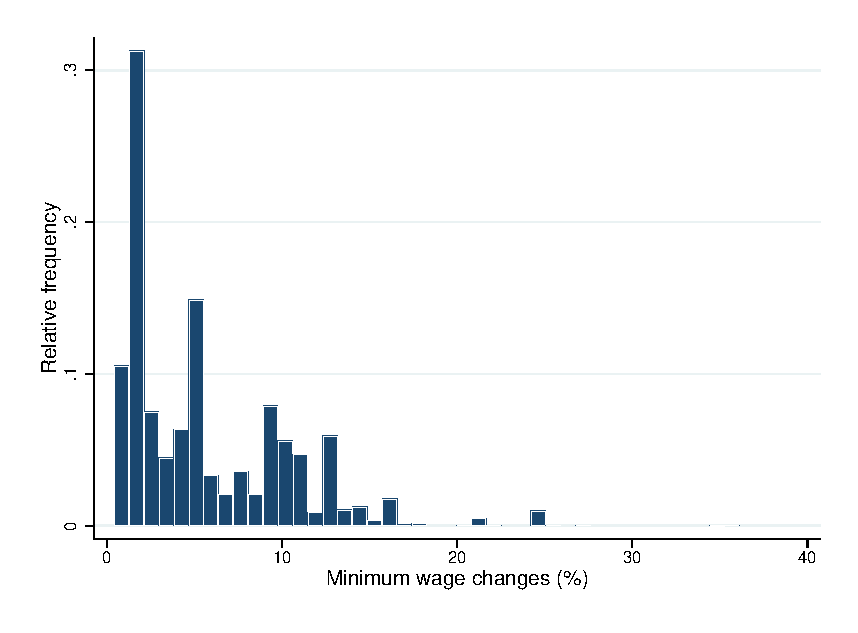
\includegraphics[width = .91\textwidth]
			{../../analysis/descriptive/output/pct_ch_mw_dist.eps}
		\end{subfigure}%
		\begin{subfigure}{.49\textwidth}
			\caption{Timing}
			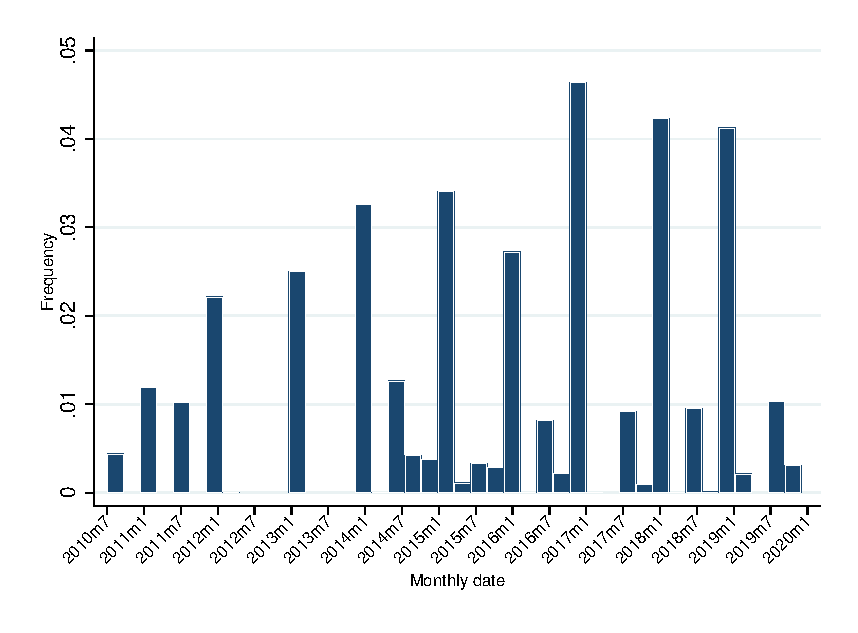
\includegraphics[width = .91\textwidth]
			{../../analysis/descriptive/output/pct_ch_mw_date_dist.eps}
		\end{subfigure}
		\begin{minipage}{.95\textwidth} \scriptsize \vspace{1mm}
			\textit{Notes:} The histograms show the distribution of positive MW changes 
			in the full sample of ZIP codes available in the Zillow data.
		\end{minipage}
	\end{figure}
	
	\hyperlink{stat_MW}{\beamerbutton{Go Back}}
\end{frame}

\begin{frame}[label=san_diego_rents]
	\frametitle{Change in rents after CA MW Increase of January 2019 in San Diego}
	
	\hyperlink{san_diego_mw}{\beamerbutton{Go Back}}
	\vspace{-7mm}
	\begin{figure} \centering
		\includegraphics[width = .48\textwidth]
			{../../analysis/descriptive_maps/output/San_Diego_rent_msa.png}
	\end{figure}
	\vspace{-7.5mm}
	\begin{minipage}{0.95\textwidth} \scriptsize
		Notes: The figure shows the change in log median rents in Zillow between December 
		2018 and June 2019.
	\end{minipage}
\end{frame}

\begin{frame}[label = dyn_alt_model]
	\frametitle{Dynamic model: Statutory MW}
	
	Adding leads and lags of the statutory MW:
	$$
	\Delta \ln r_{ict} = \delta_t
	+ \beta \Delta \underline{w}^{\text{exp}}_{ic,t+r}
	+ \sum_{r=-s}^{s} \gamma_r \Delta \ln \underline{w}_{ict}
	+ \Delta \mathbf{X}^{'}_{ct}\eta
	+ \Delta \varepsilon_{ict}
	$$
	
	where $\{\gamma_r\}_{r=-s}^{s}$ are dynamic effects of the statutory log MW.
	
	\vspace{2mm}
	\hyperlink{dyn_model}{\beamerbutton{Go Back}}
\end{frame}

\begin{frame}[label = dyn_experienced_only]
	\frametitle{Dynamic Model: Experienced log MW Only}
	\begin{figure} \centering
		\includegraphics[width = 0.6\textwidth]
		{../../analysis/first_differences_expmw/output/dynamic_exp_only_6.eps}
	\end{figure}

	\vspace{-2mm}
	\hyperlink{dyn_stat_only}{\beamerbutton{Go Back}}
\end{frame}

\begin{frame}[label = dyn_both_alt]
	\frametitle{Dynamic Model: Experienced and Statutory MW (alternative)}
	\begin{figure} \centering
		\includegraphics[width = 0.6\textwidth]
		{../../analysis/first_differences_expmw/output/dynamic_exp_and_statutory_inv_6.eps}
	\end{figure}

	\vspace{-2mm}
	\hyperlink{dyn_both}{\beamerbutton{Go Back}}
\end{frame}

\begin{frame}[label = window_size_perturbations]
	\frametitle{Window size perturbations}
	
	\begin{columns}
		\column{0.5\textwidth}
		\begin{figure}[H]
			\centering
			\includegraphics[width = \textwidth]
			{../../analysis/first_differences_expmw/output/fd_model_comparison_expmw_3.eps}
		\end{figure}
		
		\column{0.5\textwidth}
		\begin{figure}[H]
			\centering
			\includegraphics[width = \textwidth]
			{../../analysis/first_differences_expmw/output/fd_model_comparison_expmw_9.eps}
		\end{figure}
	\end{columns}

	\hyperlink{dyn_comp}{\beamerbutton{Go Back}}
\end{frame}
